\chapter{Arhitektura i dizajn sustava}

\textbf{\textit{dio 1. revizije}}\\

\section*{Uvod u Arhitekturu Sustava}
Naš sustav je dizajniran da bude efikasan, skalabilan i pouzdan. U nastavku detaljno opisujemo arhitekturu našeg sustava.

\subsection*{Izbor Arhitekture}
\begin{itemize}
    \item Naša odluka da koristimo trodijelnu arhitekturu temelji se na principima oblikovanja predstavljenim na predavanjima, gdje se ističe važnost modularnosti i odvajanja odgovornosti. Ovaj temeljni pristup oblikovanju sustava reflektira našu predanost stvaranju arhitekture koja je ne samo funkcionalna, već i prilagodljiva, jednostavna za održavanje te otporna na buduće izazove. 

    \item Princip modularnosti naglašava važnost razdvajanja sustava na manje, samostalne dijelove, ili module. Ovakav pristup omogućava da svaki modul ima jasno definiranu funkcionalnost, što pojednostavljuje razvoj, testiranje i održavanje. Svaki modul može biti razvijen neovisno, što pridonosi većoj fleksibilnosti i olakšava integraciju novih značajki ili promjena u sustavu. 

    \item Odvajanje odgovornosti, s druge strane, znači da svaki dio sustava ima precizno definiranu ulogu ili odgovornost. Na primjer, frontend se odvaja od backenda, čime se postiže jasna granica između korisničkog sučelja i poslovne logike. Ovo olakšava praćenje i održavanje svake komponente zasebno, smanjuje rizik od pogrešaka i omogućava paralelno razvijanje dijelova sustava. 

\item Trodijelna arhitektura, koja obuhvaća backend, frontend i bazu podataka, idealno se uklapa u ove principe. Backend je odgovoran za poslovnu logiku, frontend za korisničko sučelje, dok je baza podataka centralno mjesto za pohranu podataka. Ovaj pristup omogućava svakom dijelu sustava da obavlja svoju specifičnu funkciju, čime se postiže bolja organizacija, održavanje i skalabilnost. 

\subsection*{Organizacija Sustava}
\item Naš sustav je pažljivo organiziran na visokoj razini apstrakcije, koristeći klijent-poslužitelj model, što predstavlja ključni element naše arhitekture. Ova organizacija ima za cilj efikasno upravljanje različitim dijelovima sustava, pružajući jasno odvojeni pristup korisničkom sučelju i poslovnoj logici. 

\item \textbf{Klijent-poslužitelj} model je arhitektonski oblik koji omogućuje razdvajanje funkcionalnosti između dviju osnovnih komponenti: klijenta i poslužitelja. Klijent predstavlja korisničko sučelje, dok poslužitelj sadrži poslovnu logiku i podatke. Ovaj model omogućuje svakoj komponenti da obavlja svoje specifične zadatke, što rezultira modularnošću i skalabilnošću sustava. 

\textbf{Prednosti klijent-poslužitelj modela:}

\begin{enumerate}
    \item Razdvajanje odgovornosti: Klijent i poslužitelj imaju jasno definirane uloge, čime se postiže precizno odvajanje korisničkog sučelja od poslovne logike. To olakšava održavanje, poboljšava sigurnost i doprinosi boljoj organizaciji koda.
    \item Fleksibilnost i skalabilnost: Modularnost klijent-poslužitelj arhitekture omogućava prilagodbu svake komponente neovisno. Na primjer, možemo nadograditi ili zamijeniti korisničko sučelje bez narušavanja poslovne logike i obrnuto. Ovo čini sustav fleksibilnim i lako skalabilnim.
    \item Efikasna komunikacija: Klijent i poslužitelj komuniciraju putem standardiziranih protokola, često kroz HTTP. Ova jasna komunikacija omogućava brzu i pouzdanu razmjenu podataka između dijelova sustava.
\end{enumerate}
 
Odvajanje korisničkog sučelja od poslovne logike donosi dodatne prednosti. Korisničko sučelje, koje može biti web aplikacija ili mobilna aplikacija, fokusira se na prezentaciju podataka i interakciju s korisnicima. S druge strane, poslovna logika centralizirana je na poslužitelju, gdje se vrše obrade podataka, donose poslovne odluke i upravlja cjelokupnim tokom aplikacije. 

\subsection*{Detalji Podsustava}
\subsubsection*{Backend (Spring Boot)}
\item Backend predstavlja ključnu osnovu našeg sustava, pružajući infrastrukturu za obradu poslovnih zahtjeva. Organiziran je kao skup podsustava, uključujući servise i kontrolere, čija je svrha efikasno rukovanje različitim aspektima poslovnih funkcionalnosti.

\textbf{Servisi}: Funkcionalne jedinice sustava odgovorne za izvođenje specifičnih poslovnih operacija. Svaki servis fokusira se na određenu funkcionalnost, pridonoseći modularnosti i omogućavajući bolje upravljanje kompleksnošću sustava. Na primjer, možemo imati servis za korisničke operacije, proizvode ili neki drugi poslovni entitet.\newline
\textbf{Kontroleri}: Odgovorni za obradu i usmjeravanje HTTP zahtjeva koji dolaze od klijenata. Kontroleri predstavljaju sučelje između korisničkog sučelja (frontend) i poslovnih operacija koje izvode servisi. Ovo odvajanje odgovornosti omogućava bolju organizaciju koda i olakšava testiranje.



\textbf{Komunikacija s bazom podataka (PostgreSQL):}
\item Backend komunicira s bazom podataka putem PostgreSQL sustava, koji omogućava efikasnu organizaciju i manipulaciju podacima zbog svoje pouzdane i robusne arhitekture. Relacijski model podataka pruža strukturu temeljenu na tablicama, što olakšava povezivanje podataka između različitih dijelova sustava.
    \item Ovaj pristup omogućava lako preslikavanje podataka iz aplikacije u bazu i obrnuto, pridonoseći dosljednosti podataka i olakšavajući njihovo upravljanje. Kroz PostgreSQL, ostvarujemo centralno spremište podataka koje je ključno za sve relevantne informacije u sustavu.
\end{itemize}
Backend, kao središnja komponenta sustava, osigurava da poslovna logika bude učinkovito izvršavana, a podaci pravilno organizirani i održavani. Ovaj dio arhitekture pridonosi integraciji svih poslovnih funkcionalnosti, čime se postiže koherentan i efikasan rad sustava.\newline

 
 

\textbf{Frontend (Node.js, JavaScript, React)}
Frontend, kao ključna korisnička strana našeg sustava, organiziran je prema modernim principima razvoja web aplikacija. Glavni tehnološki alati koje koristimo su Node.js, JavaScript i React, pružajući nam moćne alate za stvaranje fleksibilnog i intuitivnog korisničkog sučelja.

Organizacija u komponente i kontejnere:

\begin{itemize}
    \item Komponente su modularni dijelovi koji obavljaju specifične zadatke, kao što su prikazivanje određenih podataka ili omogućavanje korisničkih interakcija.
    \item Kontejneri služe kao viši slojevi koji upravljaju komponentama, pružajući organiziran pristup i poboljšavajući skalabilnost.

\end{itemize}
REST API za komunikaciju s backendom:

\begin{itemize}
    \item Frontend komunicira s backendom putem REST API-ja (Representational State Transfer), standardnog protokola za komunikaciju između klijenta i poslužitelja koji omogućava brzu, standardiziranu i pouzdanu razmjenu podataka između frontend i backend dijelova sustava.
\end{itemize}
React kao glavni framework:

\begin{itemize}
    \item Koristimo React, popularni JavaScript framework za izgradnju korisničkih sučelja. React omogućava brzo renderiranje stranica, poboljšava učinkovitost i olakšava manipulaciju komponentama.
    \item Kroz React, frontend postaje reaktivno sučelje koje brzo reagira na promjene stanja podataka, pružajući korisnicima ugodno iskustvo korištenja aplikacije.
\end{itemize}

 

\subsubsection*{Baza podataka (PostgreSQL)}
\begin{itemize}
    \item Baza podataka predstavlja ključnu komponentu našeg sustava, pružajući centralno spremište za sve relevantne podatke. 
    \item U našem slučaju, koristimo PostgreSQL, robustan i napredan relacijski sustav upravljanja bazama podataka, kako bismo osigurali pouzdanu pohranu i učinkovit pristup podacima. 
    \item Struktura baze je dizajnirana da podržava složene upite i relacije između različitih podataka.
\end{itemize}

\subsection*{Mrežni Protokoli i Komunikacija}
\begin{itemize}
    \item Komunikacija između klijenta i poslužitelja odvija se preko HTTP protokola, osiguravajući sigurnost i standardiziran protok informacija.
    \item Kroz HTTP, klijent šalje zahtjeve poslužitelju, a poslužitelj šalje odgovore. 
\end{itemize}

\subsection*{Globalni Upravljački Tok}
\begin{itemize}
    \item Globalni upravljački tok u našem sustavu određen je kroz primjenu MVC (Model-View-Controller) arhitekture, pružajući strukturu i organizaciju za učinkovitu interakciju između različitih dijelova aplikacije. 
\end{itemize}

\textbf{MVC Arhitektura:}

\begin{itemize}
    \item \textbf{Model}: Model predstavlja središnju komponentu sustava koja upravlja podacima. Ovdje se nalaze podaci i poslovna logika aplikacije. Model je odvojen od korisničkog sučelja i interakcije te služi kao zasebna jedinica koja obrađuje podatke neovisno o korisničkom sučelju.
    \item \textbf{View}: View je odgovoran za prikazivanje podataka korisnicima. Ova komponenta generira korisničko sučelje na temelju podataka iz Modela. View je pasivan i ne obavlja izravne operacije na podacima, već ih prikazuje korisnicima na razumljiv način.
    \item \textbf{Controller}: Controller predstavlja upravljački sloj koji obrađuje korisničke zahtjeve i interakcije. Kada korisnik obavi neku akciju, Controller reagira, a zatim komunicira s Modelom i Viewom prema potrebi. Ova komponenta osigurava odvajanje korisničkih akcija od same logike sustava.

\end{itemize}
\begin{figure}[h]
    \centering
    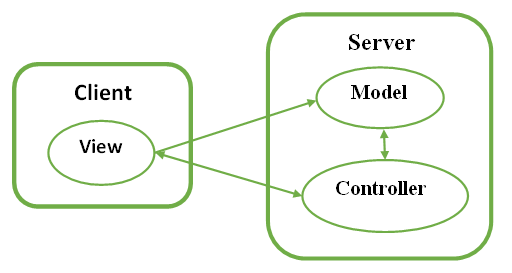
\includegraphics[width=0.5\linewidth]{slike/mvc2.png}
    \caption{MVC arhitektura}
    \label{fig:enter-label}
\end{figure}
 \textbf{
\newline Prednosti MVC Arhitekture:}
\begin{itemize}
    \item Odvajanje odgovornosti: MVC omogućava jasno odvajanje odgovornosti između različitih dijelova sustava. Model, View i Controller imaju specifične uloge, čime se olakšava razvoj, testiranje i održavanje koda.
    \item Lako proširivost i održavanje: Zbog modularnosti i odvajanja odgovornosti, dodavanje novih funkcionalnosti ili promjena postojećih dijelova sustava postaje jednostavno i manje riskantno.
    \item Jasna struktura: MVC pruža jasnu strukturu sustava, olakšavajući suradnju između različitih timova i programera. Ova organizacija doprinosi boljoj preglednosti i razumijevanju koda.
\end{itemize}

 
\subsection*{Sklopovsko-Programski Zahtjevi}
\begin{itemize}
    \item Integracijom sklopovsko-programskih zahtjeva, sustav omogućuje stabilnost te se uspješno priprema za izazove suvremenog informacijskog okruženja. 
\end{itemize}

\textbf{Prilagođenost modernim računalnim platformama:}
Sustav je optimiziran za rad na suvremenim računalnim platformama, uključujući njihove specifičnosti i prednosti. Koristeći najnovije tehnologije i prakse, osiguravamo kompatibilnost s različitim operativnim sustavima i konfiguracijama računala.\newline

\textbf{Visoka dostupnost:}
Dostupnost sustava ključna je za neprekidno pružanje usluga korisnicima. Implementiramo strategije visoke dostupnosti kako bismo osigurali minimalne prekide u radu sustava. Ovo uključuje redundanciju ključnih komponenti i mehanizme automatskog oporavka od mogućih kvarova.\newline


\textbf{Optimizacija performansi:}
Performanse su ključne za korisničko iskustvo i učinkovit rad sustava. Kroz optimizaciju koda, uporabu efikasnih algoritama i praćenje performansi u stvarnom vremenu, postižemo visoku razinu odziva i brze obrade podataka.\newline


\textbf{Prilagodljivost za skaliranje:}
Sustav je dizajniran kako bi se lako skalirao prema rastućim potrebama. Uz mogućnost horizontalnog i vertikalnog skaliranja, omogućujemo prilagodljivu infrastrukturu koja se može dinamički prilagoditi povećanju opterećenja.\newline

\textbf{Sigurnosni aspekti:}
Sklopovsko-programski zahtjevi također obuhvaćaju sigurnosne aspekte. Sustav implementira mjere zaštite podataka, enkripciju komunikacije i autentikaciju kako bi osigurao siguran rad i spriječio neovlašteni pristup.\newline


\textbf{Kontinuirano ažuriranje i praćenje trendova:}

S obzirom na brzu evoluciju tehnologije, sustav se kontinuirano prilagođava novim standardima i trendovima. Redovita ažuriranja omogućuju iskorištavanje najnovijih značajki, poboljšanje sigurnosti te održavanje konkurentske prednosti.\newline

Kroz integraciju navedenih sklopovsko-programskih zahtjeva, naš sustav ne samo da osigurava stabilnost i performanse, već je i spreman suočiti se s izazovima suvremenog informacijskog okruženja. Ovaj pristup jamči dugoročnu održivost, skalabilnost i optimalno iskorištavanje resursa računalnih platformi.

 


        \section{Baza podataka}
			
			\textbf{\textit{dio 1. revizije}}\\
			
Baza podataka predstavlja ključnu komponentu našeg sustava, pružajući centralno spremište za sve relevantne podatke. U našem slučaju, koristimo PostgreSQL, relacijski sustav upravljanja bazama podataka. PostgreSQL je snažan i visoko prilagodljiv sustav za upravljanje bazama podataka, što ga čini prikladnim izborom za učinkovito i sigurno upravljanje zdravstvenim podacima, osiguravajući da su informacije o pacijentima, terminima, zdravstvenom osoblju i opremi sigurno pohranjene i dostupne. 



\textbf{Pouzdana pohrana i pristup podacima:}

PostgreSQL pruža visoku razinu pouzdanosti i integriteta podataka. Njegova transakcijska podrška osigurava dosljednost podataka čak i u slučaju neplaniranih prekida rada sustava ili pogrešaka.
Centralizirano pohranjivanje podataka omogućava nam učinkovito upravljanje svim informacijama relevantnim za rad sustava.

\textbf{Struktura baze za složene upite i relacije:}
\begin{itemize}
\item Dizajn baze podataka ključan je za podršku složenim upitima i održavanje relacija između različitih podataka.
\item PostgreSQL, kao relacijski sustav, koristi tablice kako bi organizirao podatke. Svaka tablica sastoji se od redova i stupaca, omogućujući jasno definiranje veza između entiteta.
\item Veze između tablica omogućavaju složene upite koji spajaju informacije iz različitih dijelova sustava. 
PostgreSQL također podržava napredne mogućnosti poput indeksiranja, pomažući ubrzati upite i optimizirati performanse baze podataka.
\item  Struktura baze podataka je pažljivo oblikovana kako bi odražavala logičke relacije i potrebe sustava, čime se postiže efikasno upravljanje podacima.
\end{itemize}

		
			\subsection{Opis tablica}
			

				\textit{Svaku tablicu je potrebno opisati po zadanom predlošku. Lijevo se nalazi točno ime varijable u bazi podataka, u sredini se nalazi tip podataka, a desno se nalazi opis varijable. Svjetlozelenom bojom označite primarni ključ. Svjetlo plavom označite strani ključ}
				
\textbf{\_User } Ovaj entitet predstavlja korisnike sustava s različitim ulogama.  Sadrži atribute kao što su status korisnika (active), jedinstveni identifikator (id), e-mail adresa (email), ime (first\_name), prezime (last\_name), lozinka (password) i uloga korisnika (role). Provjerava se uloga korisnika kroz ograničenje \_user\_role\_check. Ovaj entitet omogućuje upravljanje korisnicima sustava i dodjeljivanje uloga kako bi se pristup određenim funkcionalnostima kontrolirao.  Primarni ključ (\_user\_pkey) je definiran na atributu id. 

\begin{longtblr}[
    label=none,
    entry=none
]{
    width = \textwidth,
    colspec={|X[6,l]|X[6, l]|X[20, l]|}, 
    rowhead = 1,
}
\hline \SetCell[c=3]{c}{\textbf{ \_user}} \\ \hline[3pt]
\SetCell{LightGreen}id & BIGINT & Jedinstveni identifikator korisnika \\ \hline
active & BOOLEAN & Označava je li korisnik aktivan \\ \hline 
email & VARCHAR & E-mail adresa korisnika \\ \hline 
first\_name & VARCHAR & Ime korisnika \\ \hline 
last\_name & VARCHAR & Prezime korisnika \\ \hline 
password & VARCHAR & Lozinka korisnika \\ \hline 
role & VARCHAR & Rola korisnika (mora biti jedna od predefiniranih uloga) \\ \hline 
\end{longtblr}

				
		
\textbf{Imenik} Entitet koji služi za pohranu informacija o liječnicima. Sadrži atribute kao što su jedinstveni identifikator liječnika (hlkid), ime (first\_name), prezime (last\_name), specijalizacija (specialization) i informacija o aktivnosti liječnika (active).  Primarni ključ (Imenik\_pkey) je definiran na atributu hlkid. 
\begin{longtblr}[
    label=none,
    entry=none
]{
    width = \textwidth,
    colspec={|X[6,l]|X[6, l]|X[20, l]|}, 
    rowhead = 1,
}
\hline \SetCell[c=3]{c}{\textbf{imenik}} \\ \hline[3pt]
\SetCell{LightGreen}hlkid & VARCHAR & Jedinstveni identifikator liječnika \\ \hline
first\_name & VARCHAR & Ime liječnika \\ \hline 
last\_name & VARCHAR & Prezime liječnika  \\ \hline 
specialization & VARCHAR & Specijalizacija liječnika  \\ \hline 
active & BOOLEAN & Označava je li liječnik u imeniku aktivna \\ \hline 
\end{longtblr}


\textbf{Appointment} Čuva informacije o terminima unutar sustava. Sadrži atribute kao što su datum i vrijeme termina (date\_time), identifikator zaposlenika (employee\_id), jedinstveni identifikator termina (id), identifikator pacijenta (patient\_id), identifikator sesije (session\_id), identifikator terapije (therapy\_id) i status termina (status). Ovaj entitet je povezan s drugim entitetima(employee, patient, session, therapy) putem različitih Many-to-One veza prema atributima \verb|employee_id|, \verb|patient_id|, \verb|session_id|, i \verb|therapy_id|. 

\begin{longtblr}[
    label=none,
    entry=none
]{
    width = \textwidth,
    colspec={|X[6,l]|X[6, l]|X[20, l]|}, 
    rowhead = 1,
}
\hline \SetCell[c=3]{c}{\textbf{appointment}} \\ \hline[3pt]
\SetCell{LightGreen}id & BIGINT & Jedinstveni identifikator termina \\ \hline 
date\_time & TIMESTAMP & Datum i vrijeme termina \\ \hline
\SetCell{LightBlue}employee\_id & BIGINT & Identifikator zaposlenika koji obavlja termin \\ \hline 
\SetCell{LightBlue}patient\_id & BIGINT & Identifikator pacijenta koji ima termin \\ \hline 
\SetCell{LightBlue}session\_id & BIGINT & Identifikator sesije kojoj pripada termin \\ \hline 
\SetCell{LightBlue}therapy\_id & BIGINT & Identifikator terapije koja se izvodi tijekom termina \\ \hline 
status & VARCHAR & Status termina \\ \hline 
\end{longtblr}

\textbf{Employee} Ovaj entitet predstavlja tablicu koja sadrži informacije o zaposlenicima. Sadrži atribute kao što su specijalizacija (specialization) i identifikator (id).
Ograničenje employee\_specialization\_check provjerava ispravnost specijalizacije. Primarni ključ (employee\_pkey) je definiran na atributu id. Povezan je One-to-Many vezom s entitetom session preko atributa employee\_id.

 
\begin{longtblr}[
    label=none,
    entry=none
]{
    width = \textwidth,
    colspec={|X[6,l]|X[6, l]|X[20, l]|}, 
    rowhead = 1,
}
\hline \SetCell[c=3]{c}{\textbf{employee}} \\ \hline[3pt]
\SetCell{LightGreen}id & BIGINT & Jedinstveni identifikator zaposlenika \\ \hline 
specialization & SMALLINT & Stručnost zaposlenika \\ \hline

\end{longtblr}

\textbf{Equipment} Ovaj entitet predstavlja tablicu koja sadrži informacije o opremi. Svaka oprema ima svoj jedinstveni identifikator (id) za precizno praćenje. Attribut capacity označava kapacitet opreme, dok description pruža dodatne opise ili karakteristike. Naziv opreme (name) jedinstveno označava svaki komad, olakšavajući identifikaciju i korištenje unutar medicinskog okruženja. 
\begin{longtblr}[
    label=none,
    entry=none
]{
    width = \textwidth,
    colspec={|X[6,l]|X[6, l]|X[20, l]|}, 
    rowhead = 1,
}
\hline \SetCell[c=3]{c}{\textbf{equipment}} \\ \hline[3pt]
\SetCell{LightGreen}id & BIGINT & Jedinstveni identifikator opreme \\ \hline 
capacity & INTEGER & Kapacitet opreme \\ \hline
description & VARCHAR & Opis opreme \\ \hline 
name & VARCHAR & Naziv opreme \\ \hline 
\end{longtblr}

\textbf{Patient} Ovaj entitet predstavlja tablicu  koja sadrži informacije o pacijentima.  Sadrži atribute kao što su datum rođenja, identifikator (id), adresa, MBO (matični broj osiguranika) i broj telefona. Primarni ključ (patient\_pkey) je definiran na atributu id.
 
\begin{longtblr}[
    label=none,
    entry=none
]{
    width = \textwidth,
    colspec={|X[7,l]|X[6, l]|X[19, l]|}, 
    rowhead = 1,
}
\hline \SetCell[c=3]{c}{\textbf{patient}} \\ \hline[3pt]
\SetCell{LightGreen}id & BIGINT & Jedinstveni identifikator pacijenta \\ \hline 
date \_of\_birth & DATE & Datum rođenja pacijenta \\ \hline
address & VARCHAR & Adresa pacijenta \\ \hline 
mbo & VARCHAR & Matični broj osiguranika pacijenta \\ \hline 
phone\_number & VARCHAR & Broj telefona pacijenta \\ \hline 
\end{longtblr}

\textbf{Session} Ovaj entitet predstavlja tablicu koja sadrži informacije o sesijama.  Sadrži atribute kao što su datum i vrijeme, identifikator zaposlenika, identifikator sesije i povratna informacija (feedback). Primarni ključ (session\_pkey) je definiran na atributu id. Povezan je Many-to-One vezom s entitetom employee preko atributa employee\_id. 
\begin{longtblr}[
    label=none,
    entry=none
]{
    width = \textwidth,
    colspec={|X[6,l]|X[6, l]|X[20, l]|}, 
    rowhead = 1,
}
\hline \SetCell[c=3]{c}{\textbf{session}} \\ \hline[3pt]
\SetCell{LightGreen}id & BIGINT & Jedinstveni identifikator sesije \\ \hline
date\_time & timestamp & Vrijeme sesije \\ \hline 
\SetCell{LightBlue}employee\_id & BIGINT & Identifikator zaposlenika \\ \hline 
feedback & character varying(255) & Povratna informacija o sesiji \\ \hline 
\end{longtblr}


\textbf{Therapy}  Ovaj entitet predstavlja tablicu koja sadrži informacije o terapijama.  Sadrži atribut identifikator (id) i atribut therapy\_type\_id. Primarni ključ (therapy\_pkey) je definiran na atributu id.  Također sadrži jedinstveno ograničenje therapy\_therapy\_type\_id\_key na atributu therapy\_type\_id. Povezan je One-to-One vezom s entitetom appointment preko atributa therapy\_id.
\begin{longtblr}[
    label=none,
    entry=none
]{
    width = \textwidth,
    colspec={|X[7,l]|X[6, l]|X[19, l]|}, 
    rowhead = 1,
}
\hline \SetCell[c=3]{c}{\textbf{therapy}} \\ \hline[3pt]
\SetCell{LightGreen}id & BIGINT & Jedinstveni identifikator terapije \\ \hline
\SetCell{LightBlue}therapy\_type\_id & BIGINT & Identifikator vrste terapije \\ \hline 
\end{longtblr}

\textbf{Therapy\_type} Ovaj entitet predstavlja tablicu koja sadrži informacije o vrstama terapija. Sadrži atribute kao što su identifikator (id), identifikator potrebne opreme (required\_equipment\_id) i opis. Primarni ključ (therapy\_type\_pkey) je definiran na atributu id. Povezan je Many-to-One vezom s entitetom therapy preko atributa required\_equipment\_id i s entitetom equipment preko atributa required\_equipment\_id. 
\begin{longtblr}[
    label=none,
    entry=none
]{
    width = \textwidth,
    colspec={|X[10,l]|X[6, l]|X[17, l]|}, 
    rowhead = 1,
}
\hline \SetCell[c=3]{c}{\textbf{therapy\_type}} \\ \hline[3pt]
\SetCell{LightGreen}id & BIGINT & Jedinstveni identifikator vrste terapije \\ \hline
\SetCell{LightBlue}required\_equipment\_id & BIGINT & Identifikator potrebnog opreme \\ \hline 
description & character varying(255) & Opis vrste terapije \\ \hline 
\end{longtblr}
				
			
			\subsection{Dijagram baze podataka}
        Svaka tablica ima primarni ključ koji jedinstveno identificira zapise unutar tablice. Baza podataka uspostavlja odnose između tablica koristeći strane ključeve. Ograničenja su postavljena kako bi se očuvao integritet podataka.  
			
    \begin{figure}[h]
			    \centering
			    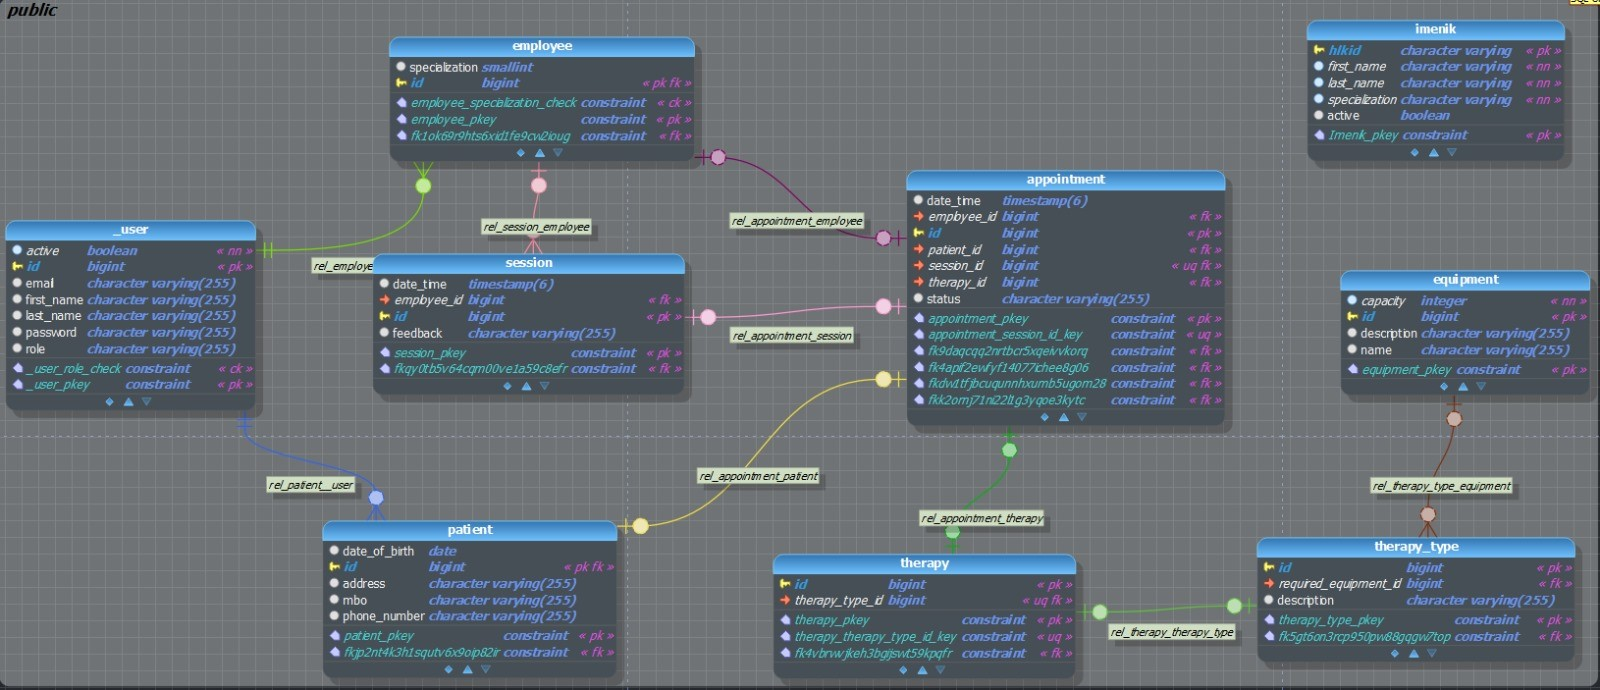
\includegraphics[width=1\linewidth]{slike/database_pr1.jpg}
			    \caption{Dijagram baze podataka}
			    
			    \label{fig:enter-label}
			\end{figure}
			\eject
			
			
		\section{Dijagram razreda}
		
		

            
      

    Dijagram razreda  prikazan je  na slici 4.3.  Implementirane metode direktno komuniciraju s bazom podataka te vraćaju tražene podatke  poput popisa dijelatnika, opreme, provjere je li dijelatnik i dalje aktivan.
	

Razredi Employee i Patient  generalizacija su razreda User pa nasljeđuju njegove public atribute i metode.
Razred User predstavlja osnovni model korisnika u sustavu. Ovaj razred obuhvaća osnovne informacije o korisniku, uključujući ime, prezime, korisničko ime profila, email adresu, lozinku i status aktivnosti korisničkog računa. Dodatno, svaki korisnik ima dodijeljenu ulogu koja se koristi za upravljanje ovlastima unutar sustava, a ta uloga je opisana pomoću enumeracije putem razreda  Role.
Razred Employee predstavlja model zaposlenika u medicinskom sustavu. Proširuje osnovni razred User, dodajući specifične atribute i odnose relevantne za zaposlenike u sustavu.  Razred Patient predstavlja model pacijenta u medicinskom sustavu. 
Razred Specialization predstavlja enumeraciju koja sadrži različite vrste specijalizacija dijelatnika u medicinskom sustavu. 
Razred Session predstavlja radnu sesiju unutar medicinskog sustava. Ovaj razred omogućuje praćenje sesija između zaposlenika i pacijenata. 
 Zahtjev za terapijom se sastavlja pomoću  vrste terapije i identifikatora pacijenta, zaposlenika i terapije.
Razred Equipment predstavlja opremu koja se koristi u medicinskom sustavu. Ovaj razred pruža informacije o različitim vrstama opreme, uključujući jedinstveni identifikator opreme, kapacitet, opis i naziv opreme. 
Razred Therapy predstavlja terapiju unutar medicinskog sustava. 
Razred TherapyType predstavlja vrstu terapije u sustavu. \\

\begin{figure}[H]
    \centering
    
\includegraphics[width=0.5\linewidth]{slike/dijagramRazredaFinal.png}
    \caption{Dijagram razreda}
    \label{fig:enter-label}
\end{figure}



Svaki od ovih entiteta slijedi obrazac  \verb|Controller -> Service -> Repository| za obavljanje operacija nad podacima.

Na primjer, entitet Employee posjeduje EmployeeController, EmployeeService i EmployeeRepository. Ovi razredi zajednički omogućuju upravljanje informacijama o zaposlenicima, uključujući njihovu autentikaciju. Kroz ovaj ciklus, Controller komunicira s Servisom, a Servis dalje s Repozitorijem, osiguravajući konzistentan i siguran pristup podacima.

Osim toga, entiteti poput Therapy, Appointment i Session imaju svoje setove Controllera, Servisa i Repozitorija koji omogućuju operacije vezane uz terapije, narudžbe pacijenata i sesije.

Bitna karakteristika ovog organiziranog pristupa je da Controller vraća odgovarajući HTTP status i tražene informacije (klasa, string ili ništa) u obliku JSON-a. Ovaj proces olakšava komunikaciju između različitih dijelova sustava, pružajući jasnu i strukturiranu komunikaciju među različitim slojevima aplikacije.

Kad Patient izvrši registraciju ili prijavu, procesi autentikacije i autorizacije upravljaju se putem SecurityControllera i SecurityServicea. Ovi kontroleri i servisi surađuju s SecurityConfig-om, implementiranim pomoću WebConfig, kako bi provjerili je li pacijent, administrator ili zdravstveni djelatnik autoriziran i autentificiran za svaku radnju koju žele izvršiti u sustavu.

SecurityController omogućuje upravljanje zahtjevima vezanim uz sigurnost, poput registracije i prijave korisnika, dok SecurityService sadrži logiku autentikacije i autorizacije. Ove komponente zajednički rade kako bi osigurale siguran pristup podacima i funkcionalnostima sustava.

Kroz SecurityConfig i WebConfig, postavke sigurnosti konfiguriraju se prema tipu korisnika. Ovaj postupak osigurava da pacijenti, administratori i zdravstveni djelatnici imaju odgovarajuće privilegije za izvršavanje željenih radnji, uzimajući u obzir autentikaciju i autorizaciju.

Ova struktura omogućuje efikasno i sigurno upravljanje pristupom resursima u sustavu, osiguravajući da svaki korisnik ima odgovarajuće ovlasti za obavljanje svojih funkcija u skladu s postavljenim sigurnosnim pravilima.\\

 

 

 

  

 
			
			
			
			\eject
		
		\section{Dijagram stanja}
			

   Dijagram stanja za registriranog i prijavljenog korisnika(pacijenta) prikazan je na Slici 4.4. Početno stanje označava da je korisnik već uspješno prijavljen u sustav te se preusmjerava na dashboard s rasporedom terapija. Ovdje korisnik može vidjeti trenutnu terapiju koja mu je dodijeljena.


U gornjem desnom kutu nalaze se gumbići za pristup korisničkom profilu pacijenta, kreiranje nove terapije ili odjavu. Klikom na korisnički profil, korisnik može pregledati osobne podatke i bilješke liječnika o terapijama. Također, korisnik ima mogućnost ažuriranja svojih osobnih podataka, uključujući promjenu broja mobitela ili postavljanje nove profilne slike. Odabirom opcije "New Therapy", korisnik može unijeti kod ili odabrati dio tijela sa skice za koji želi terapiju. Nakon toga, prikazuje se kalendar s dostupnim terminima za odabranu terapiju, gdje korisnik bira jedan ili više termina. Slanjem zahtjeva s MBO-om, šifrom terapije i odabranim datumom, korisnik podnosi zahtjev za novom terapijom.

U gornjem desnom kutu smješteni su gumbi koji omogućavaju prijelaz u tamni način rada te promjenu jezika između engleskog i hrvatskog, čime se postiže dvojezičnost u našoj aplikaciji.

Na dnu stranice smješten je virtualni asistent. MedBot je zadužen za pružanje općih informacija o terapijama, dok BayBot odgovara na pitanja korisnika vezana uz korištenje aplikacije.

Korisnik također ima opciju odjave, što vodi u završno stanje. U svakom trenutku korisnik može i deaktivirati račun.
			
			\begin{figure}[H]
			    \centering
			    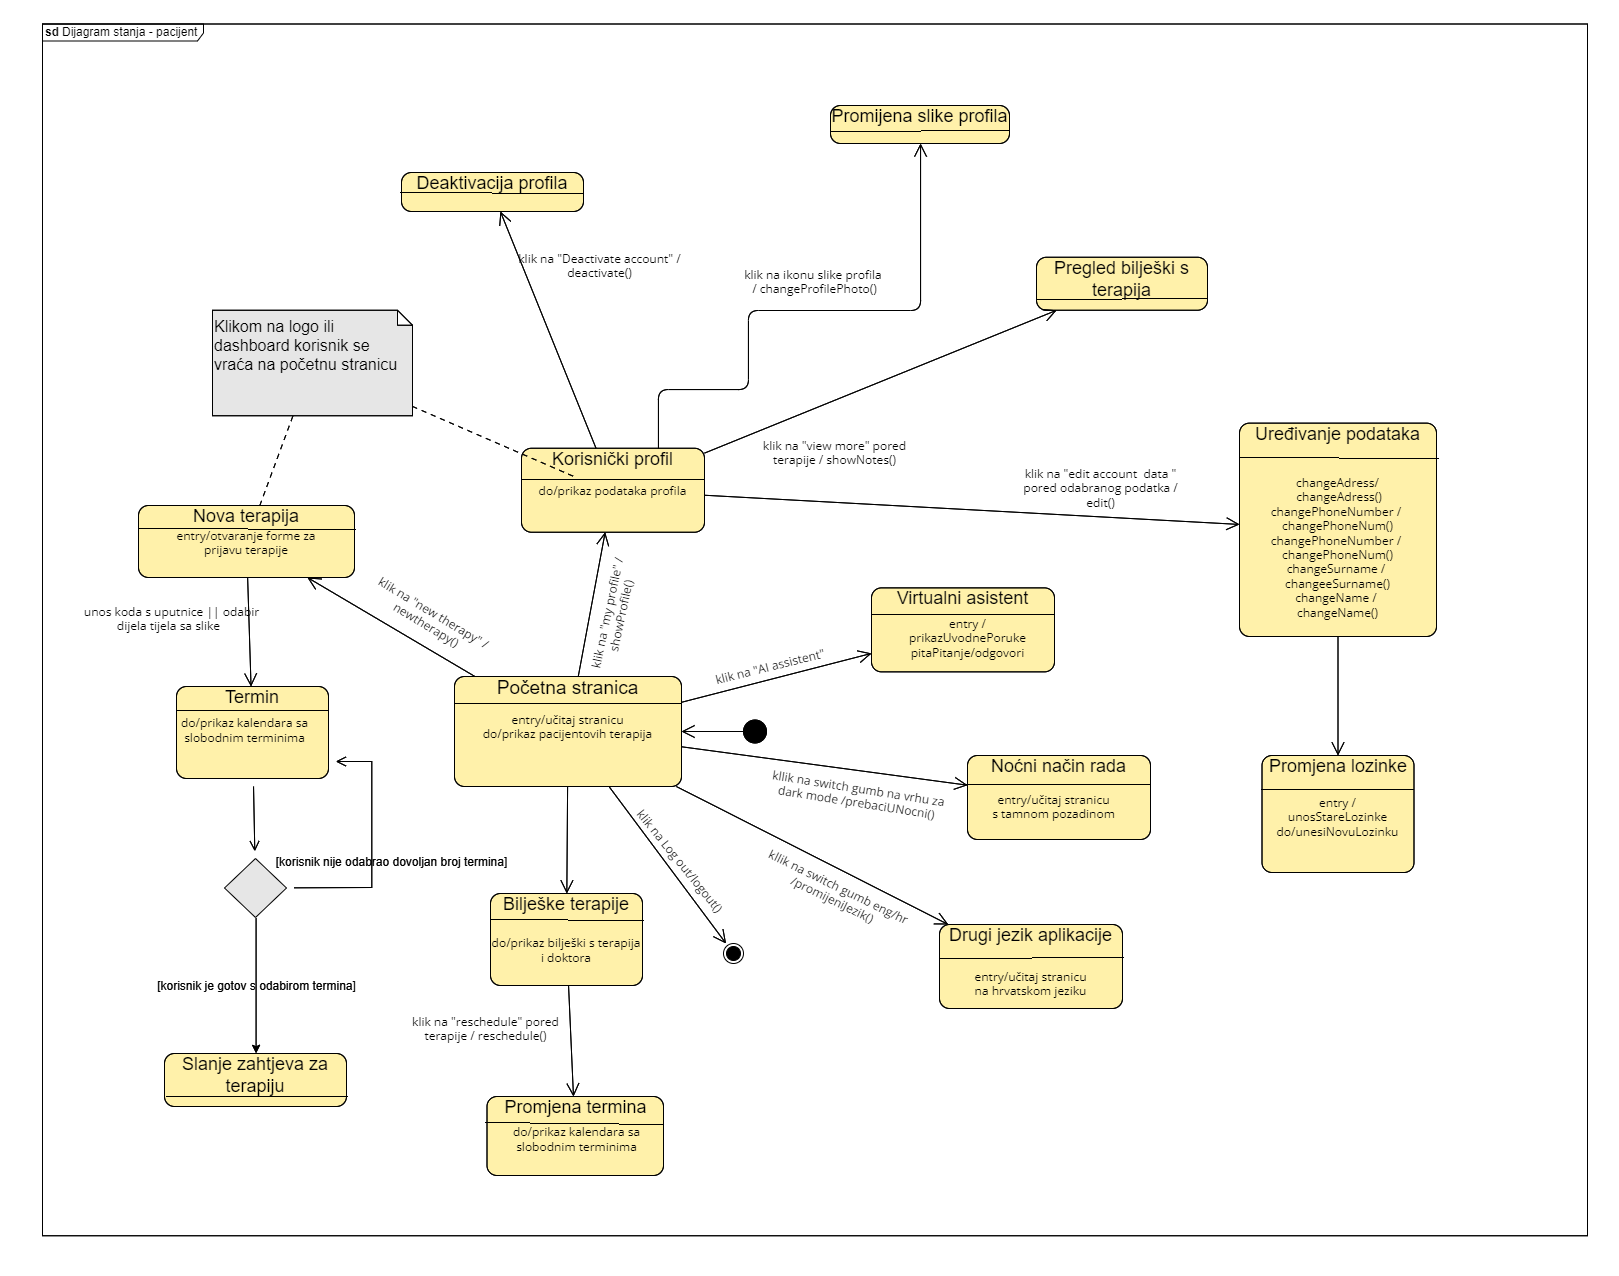
\includegraphics[width=1\linewidth]{slike/dijStanjaFinal.png}
			    \caption{Dijagram stanja - pacijent}
			    \label{fig:enter-label}
			\end{figure}
			\eject 
		
		\section{Dijagram aktivnosti}
			

            Na dijagramu aktivnosti 4.5 prikazan je proces kreiranja nove terapije. Korisnik (pacijent) se prijavljuje u sustav. 
            Bira opciju za kreiranje nove terapije, unosi kod terapije ili bira iz dostupnih opcija.
            Odabire termine na kalendaru, unosi broj uputnice i identifikacijski broj liječnika.
            Nakon unosa svih podataka, korisnik klikne na gumb "Završi" čime se zahtjev šalje administratoru na odobrenje.            
            
            \begin{figure}[H]
             \centering
             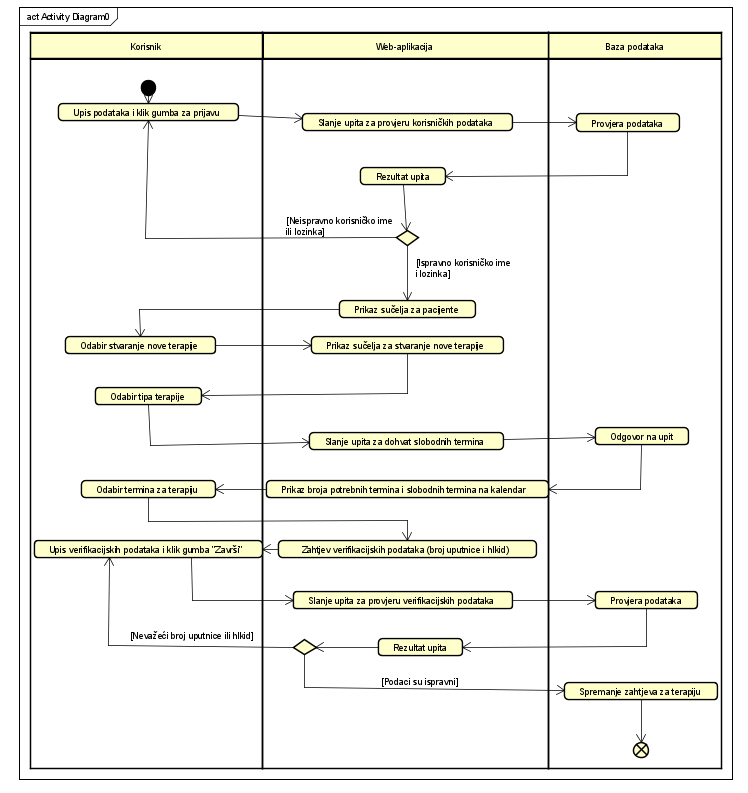
\includegraphics[width=1\linewidth]{slike/dijagramAktivnosti.png}
             \caption{Dijagram aktivnosti}
             \end{figure}
			\eject

		\section{Dijagram komponenti}
			
			\textbf{\textit{dio 2. revizije}}\\
			

            Dijagram komponenti prikazuje od kojih komponenti je sustav sastavljen, kako te komponente međusobno surađuju i ovise jedna o drugoj. Iz sustava se informacije dobivaju na dva načina: upitima \textit{frontendu} i \textit{backendu}. \textit{Frontend} dio (HTML, CSS, JS) dohvaća se preko datoteke App.jsx koja vodi brigu o tome što će se prikazati. App.jsx ovisan je o bibliotekama Reacta. \textit{Frontend} u sebi sadrži segmente koji mogu poslati podatke \textit{backendu} na obradu. Tu \textit{backend} prima zahtjeve s određenim podatcima, analizira ih kroz \textit{Controllere}, Servise i Repozitorije (zadnji komunicira s PostgreSQL bazom podataka). Na taj način korisnik dobiva sučelja i informacije koje se njega tiču.
            
            \begin{figure}[H]
             \centering
             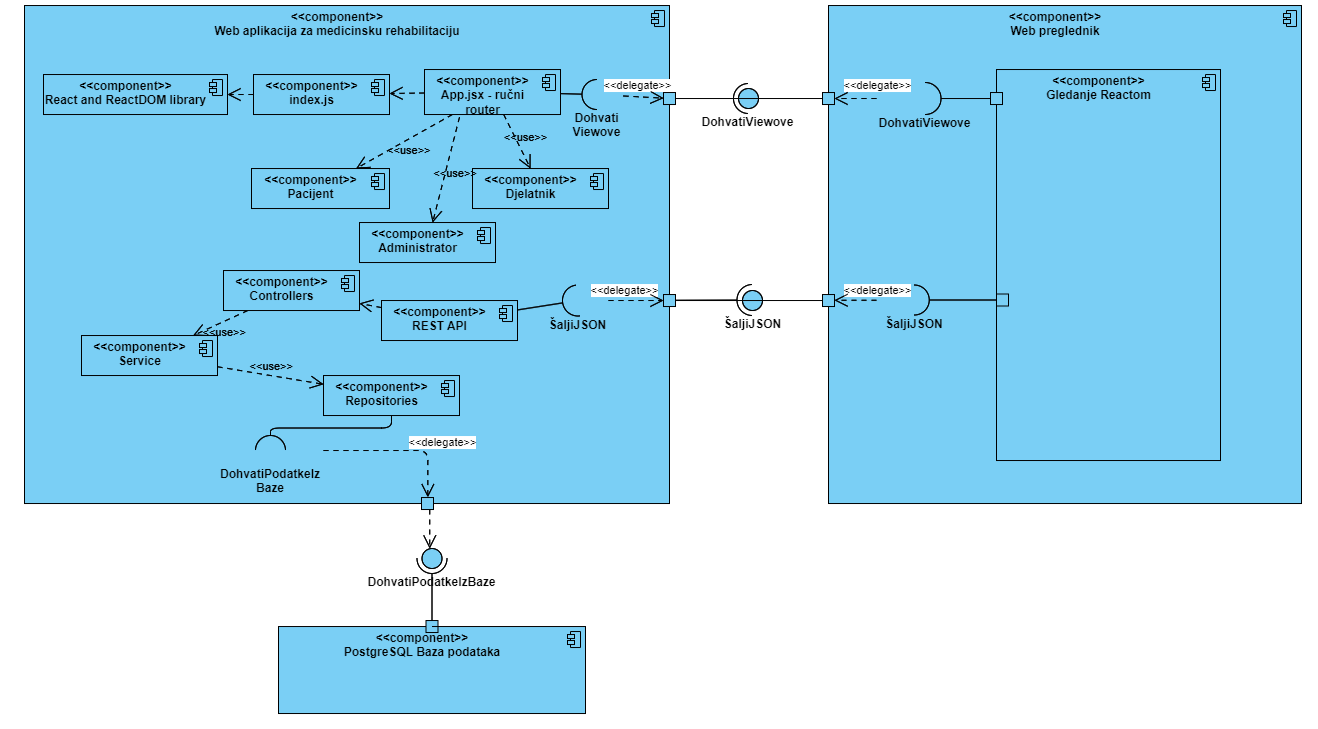
\includegraphics[width=1\linewidth]{slike/dijagramKomponenti.png}
             \caption{Dijagram komponenti}
             \end{figure}
			\eject 
